\renewcommand{\thefigure}{S\arabic{figure}}
\renewcommand{\thetable}{S\arabic{table}}

%%%%%%%%%%%%%%%%%%%%%%%%%%%%%%%%%%%%%%%%%% FIGURE
\begin{figure*}   
  \begin{center}
   \vspace{-0mm}
   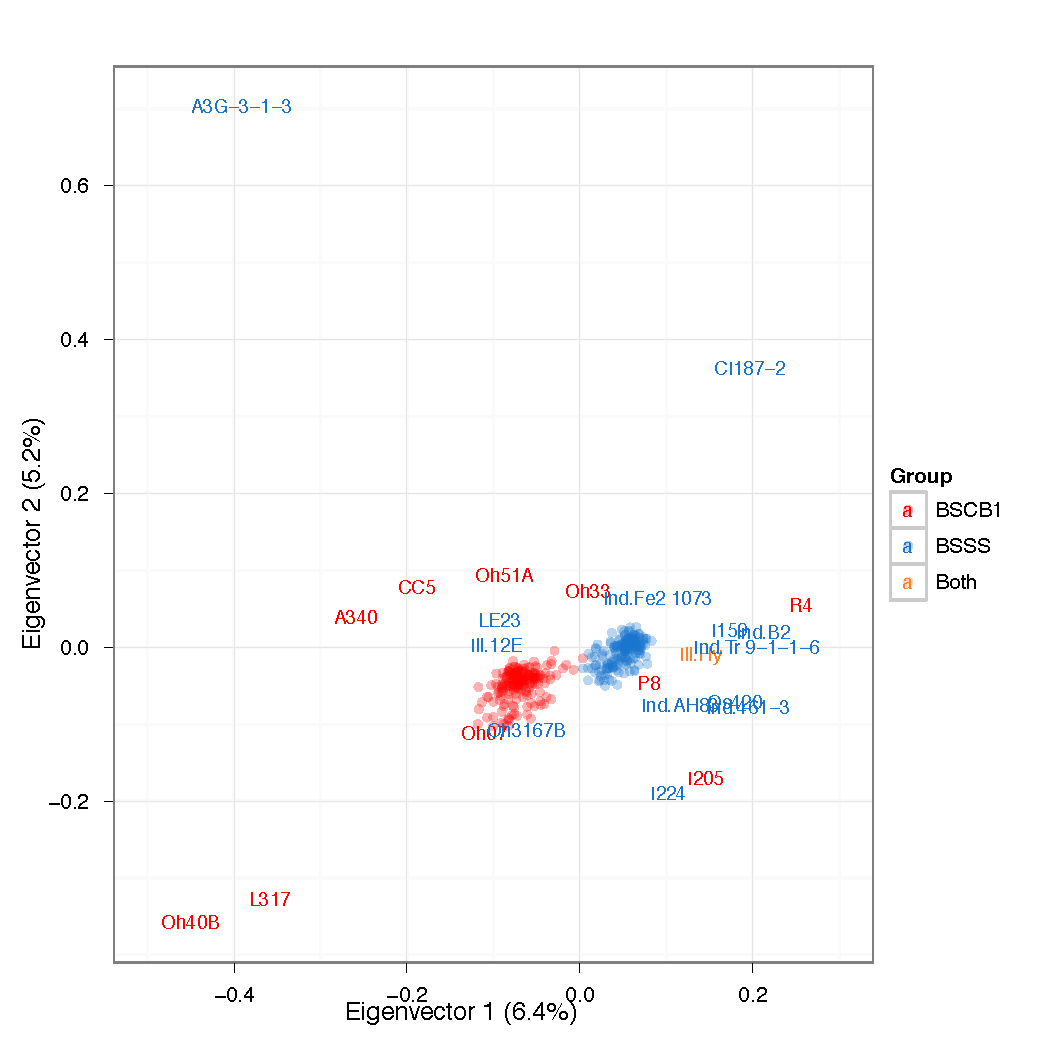
\includegraphics[width=0.7\linewidth]{pca_founders}
   %\renewcommand{\baselinestretch}{0.9}
   \vspace{-3mm}
   \caption{ Principle component analysis of founder inbred lines. The names of founder inbreds are shown on the graph; all other points represent BSSS (blue) and BSCB1 (red) individuals projected onto the PCA of the founders.
} 
\vspace{-6mm}
    \label{fig:sfounders}
  \end{center}
\end{figure*}
%%%%%%%%%%%%%%%%%%%%%%%%%%%%%%%%%%%%%%%%%% FIGURE


%%%%%%%%%%%%%%%%%%%%%%%%%%%%%%%%%%%%%%%%%% FIGURE
\begin{figure*}   
  \begin{center}
   \vspace{-0mm}
   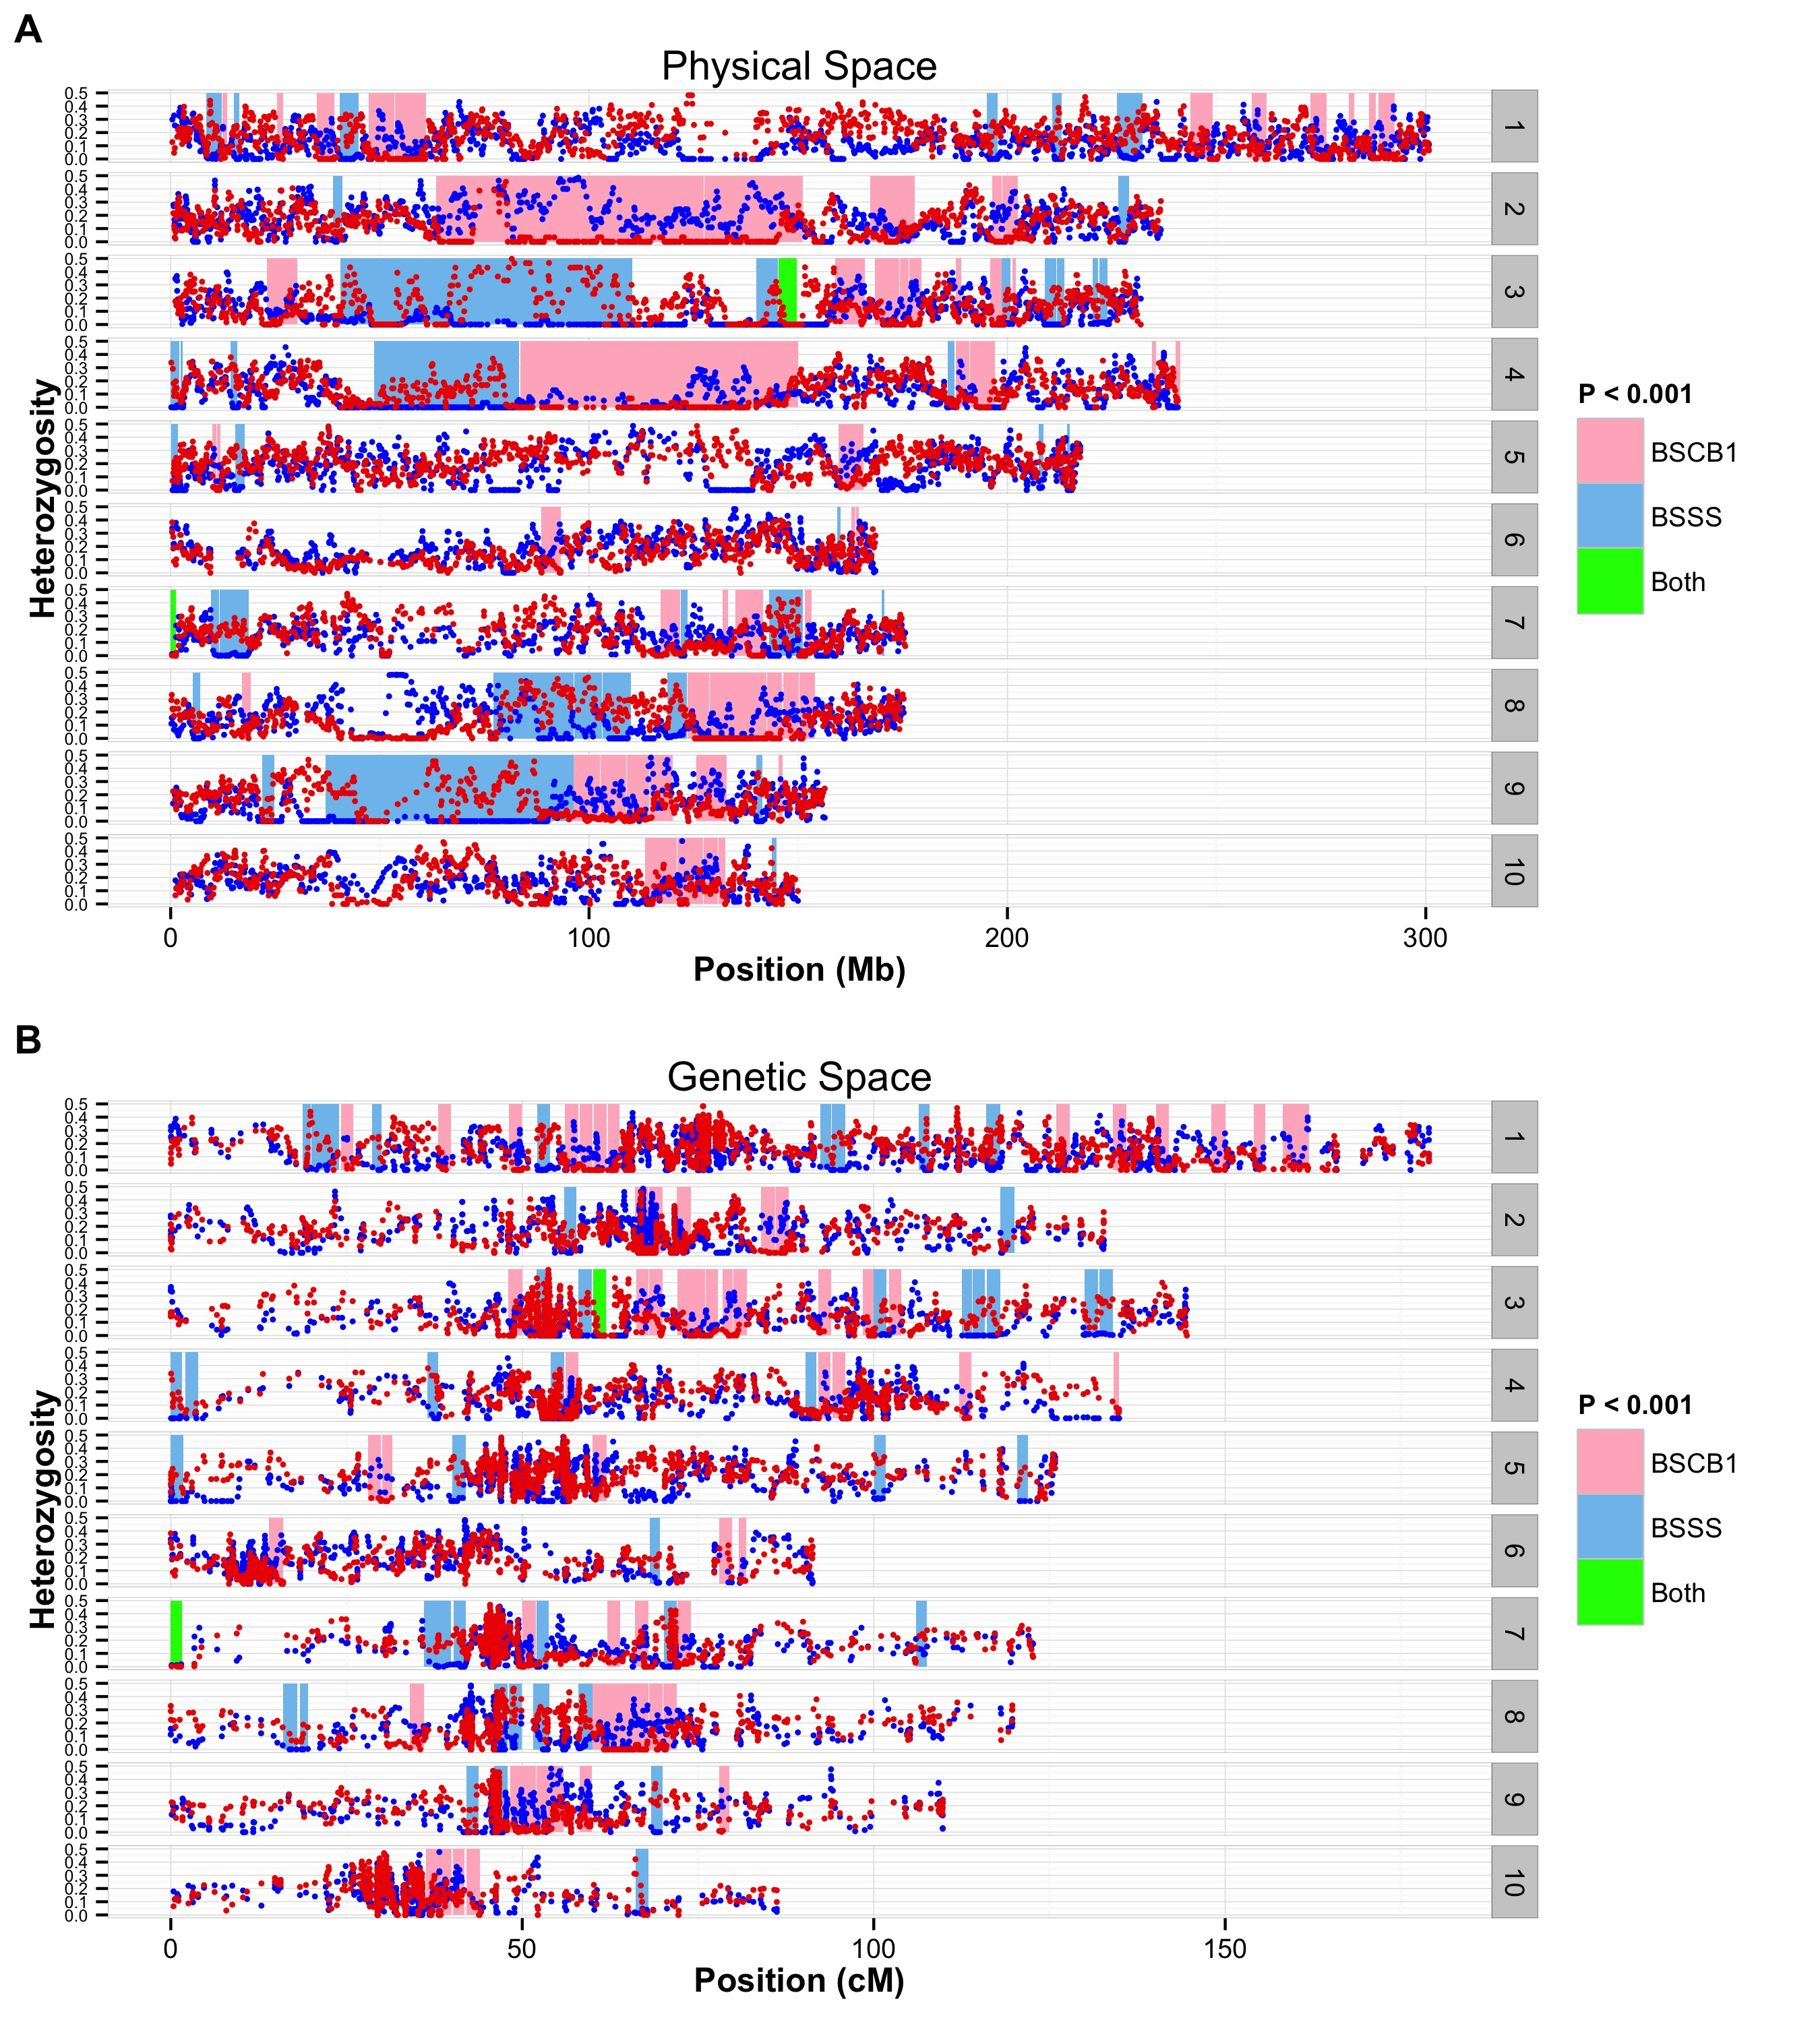
\includegraphics[width=0.7\linewidth]{fig3}
   %\renewcommand{\baselinestretch}{0.9}
   \vspace{-3mm}
   \caption{ Heterozygosity ($H$) at cycle16 across all ten chromosomes in each population.  $H$ is calculated on 15-marker sliding windows with 5 marker steps. Each point is plotted at the midpoint of the 15-marker window. 
} 
\vspace{-6mm}
    \label{fig:s2}
  \end{center}
\end{figure*}
%%%%%%%%%%%%%%%%%%%%%%%%%%%%%%%%%%%%%%%%%% FIGURE

%%%%%%%%%%%%%%%%%%%%%%%%%%%%%%%%%%%%%%%%%% FIGURE
\begin{center}
\Image[width=0.7\linewidth]{Fig4/chrom1_combined}{} \\
\Image[width=0.7\linewidth]{Fig4/chrom2_combined}{} 
\newpage
\Image[width=0.7\linewidth]{Fig4/chrom3_combined}{} \\
\Image[width=0.7\linewidth]{Fig4/chrom5_combined}{} 
\newpage
\Image[width=0.7\linewidth]{Fig4/chrom6_combined}{} \\
\Image[width=0.7\linewidth]{Fig4/chrom7_combined}{} 
\newpage
\Image[width=0.7\linewidth]{Fig4/chrom8_combined}{} \\
\Image[width=0.7\linewidth]{Fig4/chrom9_combined}{} 
\newpage
\Image[width=0.7\linewidth]{Fig4/chrom10_combined}{}  
\captionof{figure}{Heterozygosity in each cycle across chromosomes of the BSSS (left) and BSCB1 (right) plotted on the physical (top) and genetic (bottom) map. Details are as in Fig. 4.}
    \label{fig:others2}
\end{center}




%\begin{figure*}   
%  \begin{center}
%   \vspace{-0mm}
%   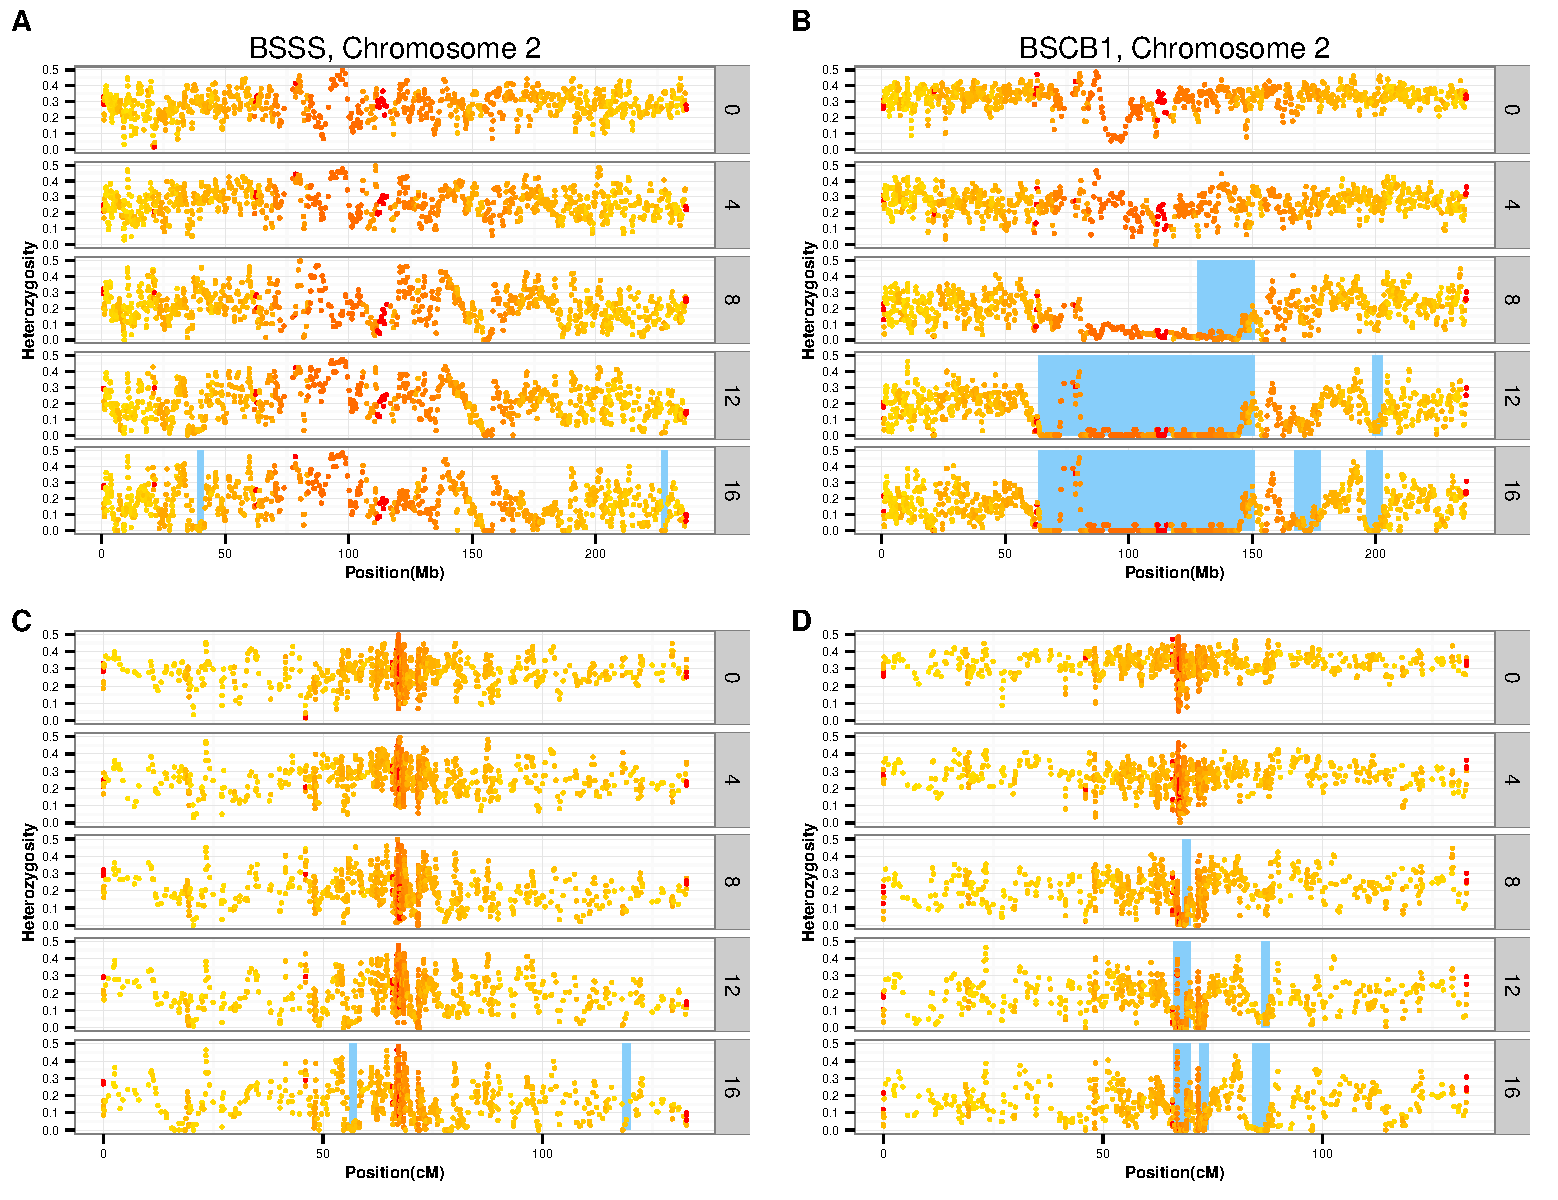
\includegraphics[width=0.7\linewidth]{Fig4/chrom2_combined.pdf}
%   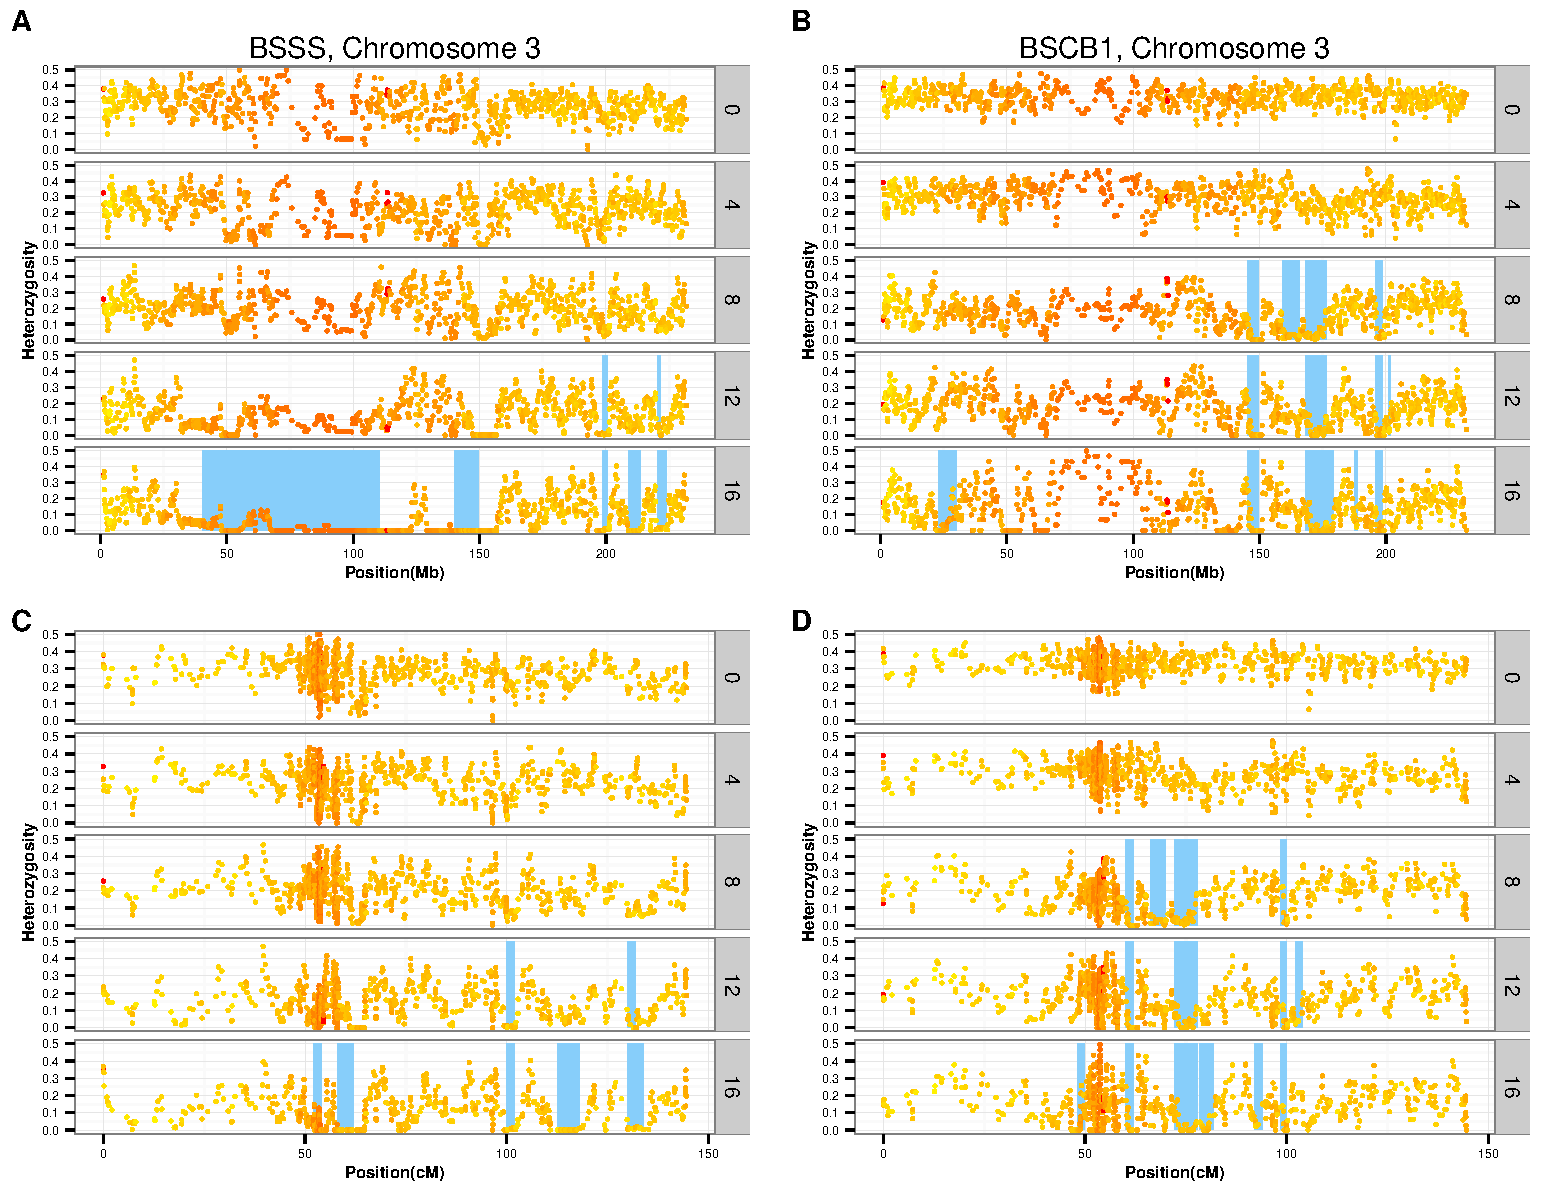
\includegraphics[width=0.7\linewidth]{Fig4/chrom3_combined.pdf}
%   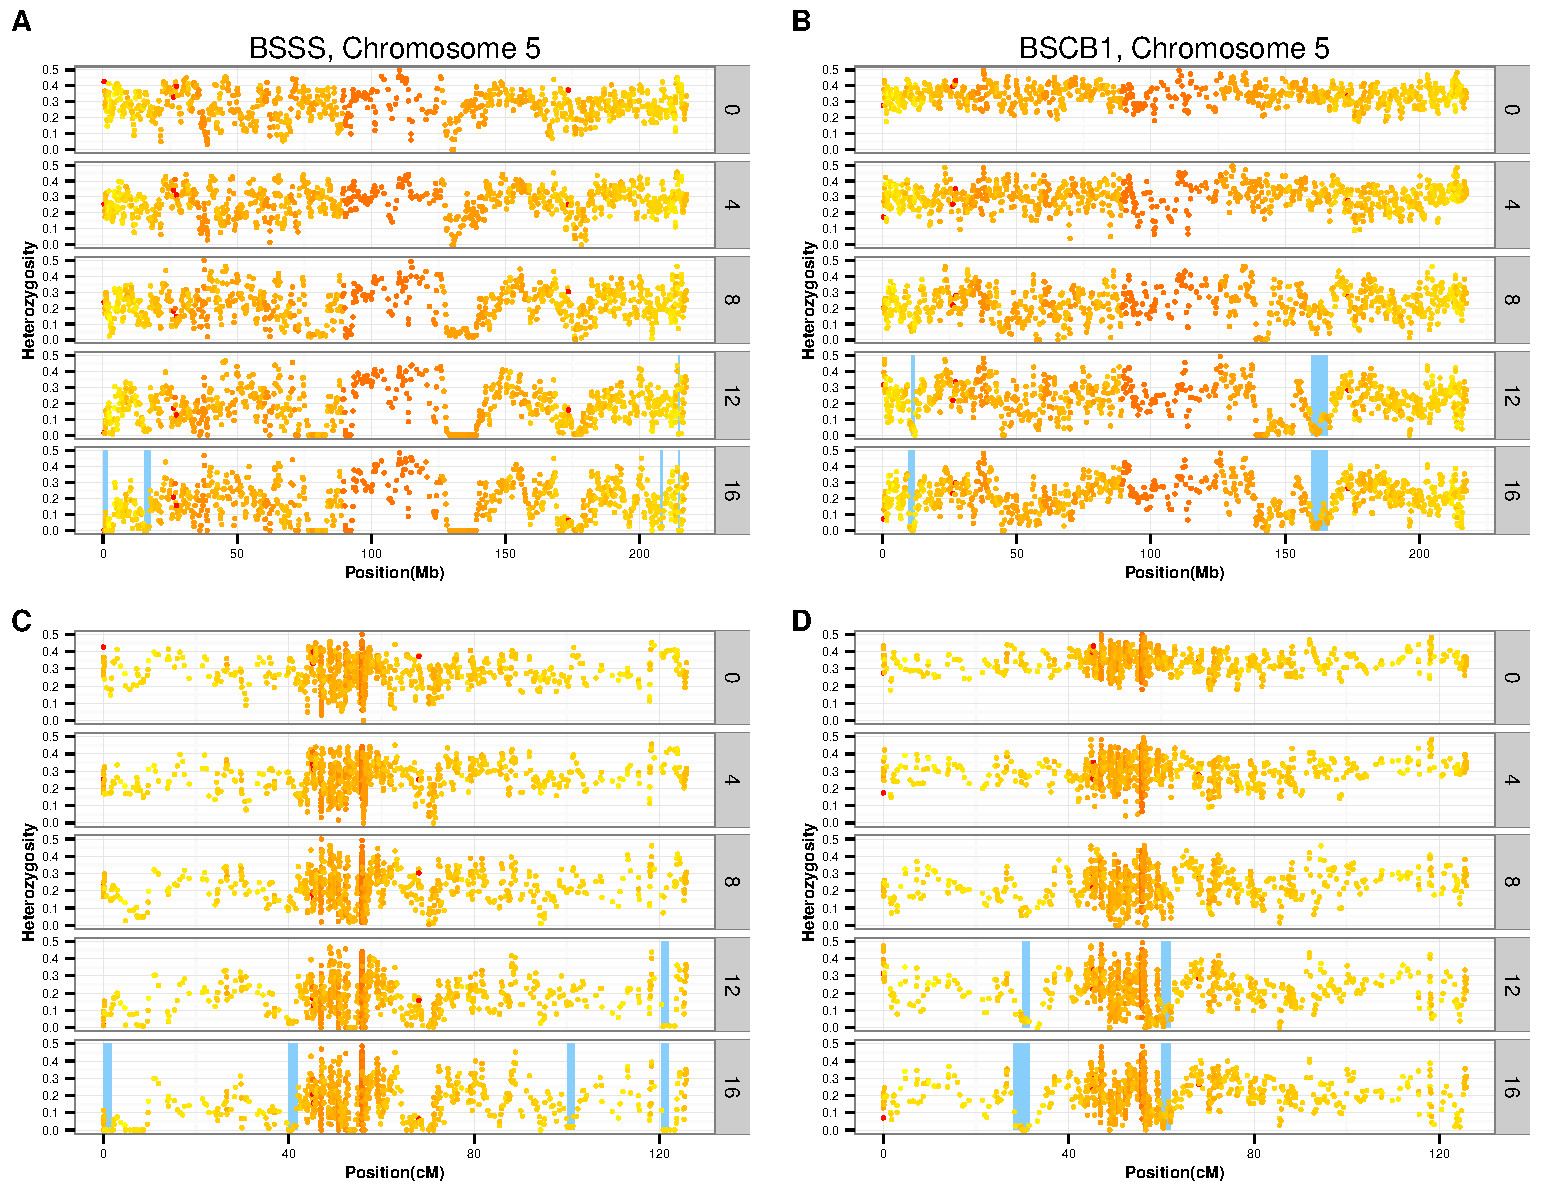
\includegraphics[width=0.7\linewidth]{Fig4/chrom5_combined.pdf}
%   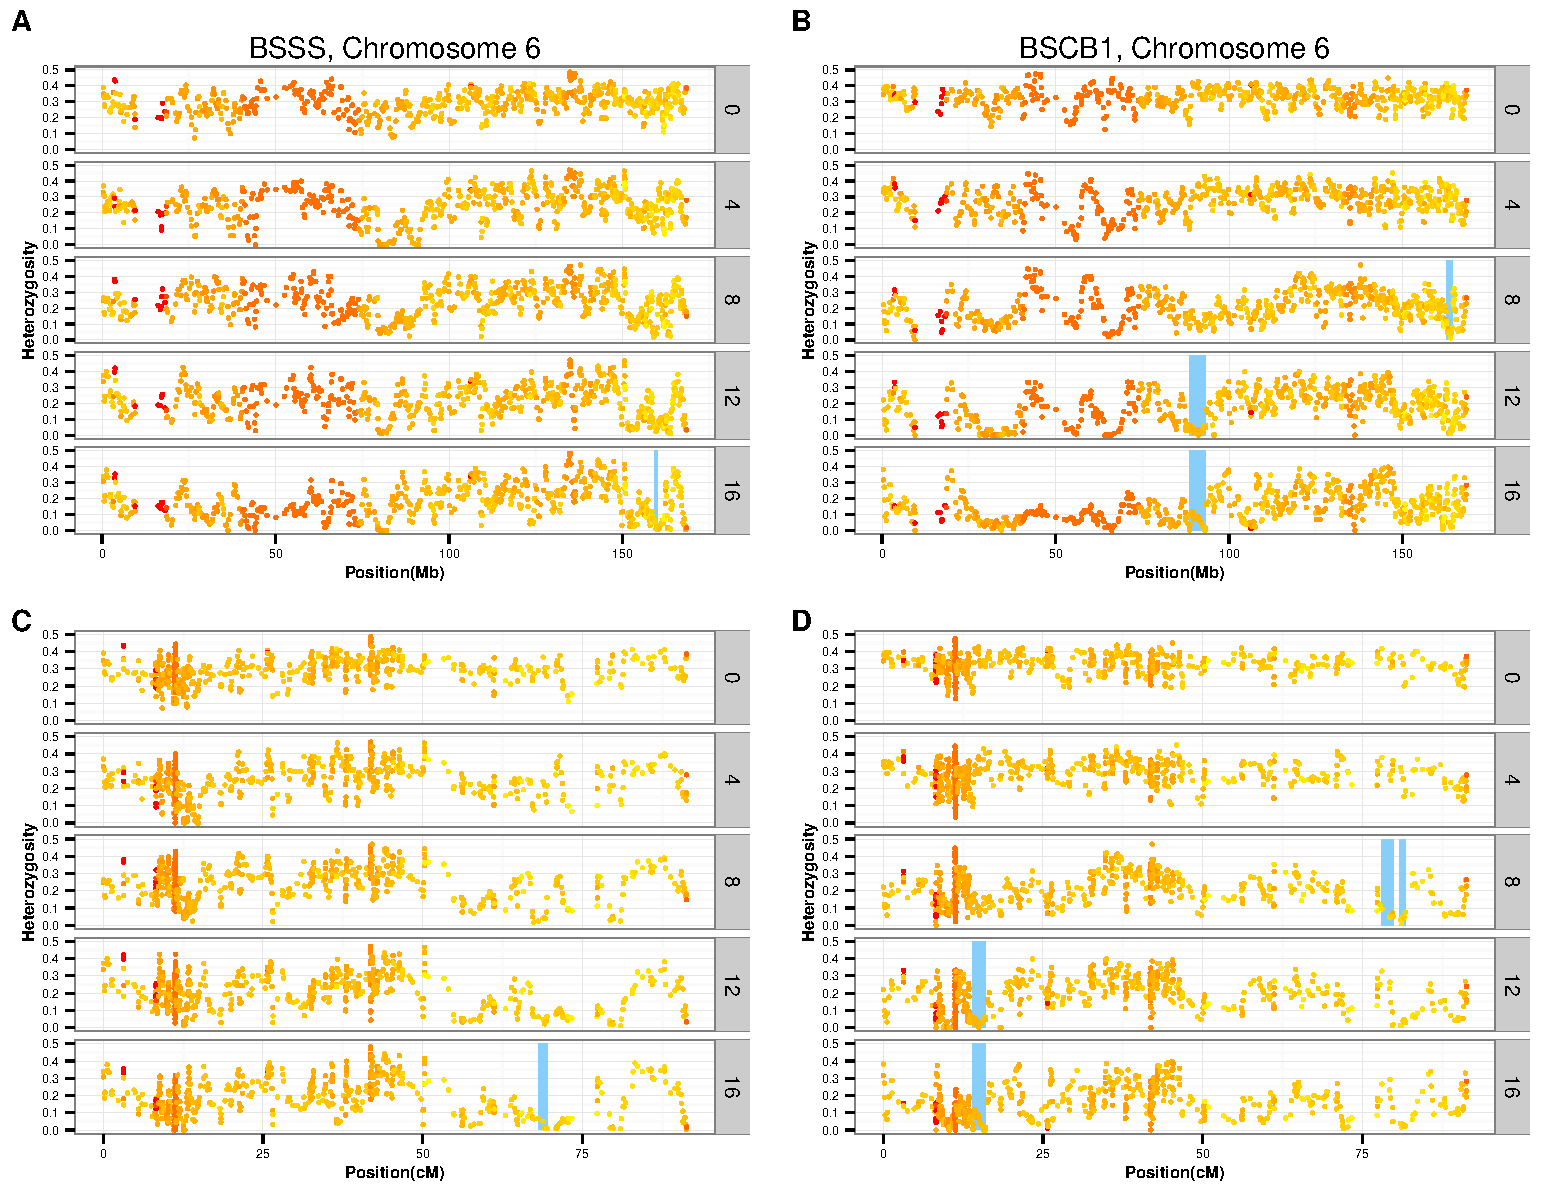
\includegraphics[width=0.7\linewidth]{Fig4/chrom6_combined.pdf}
%   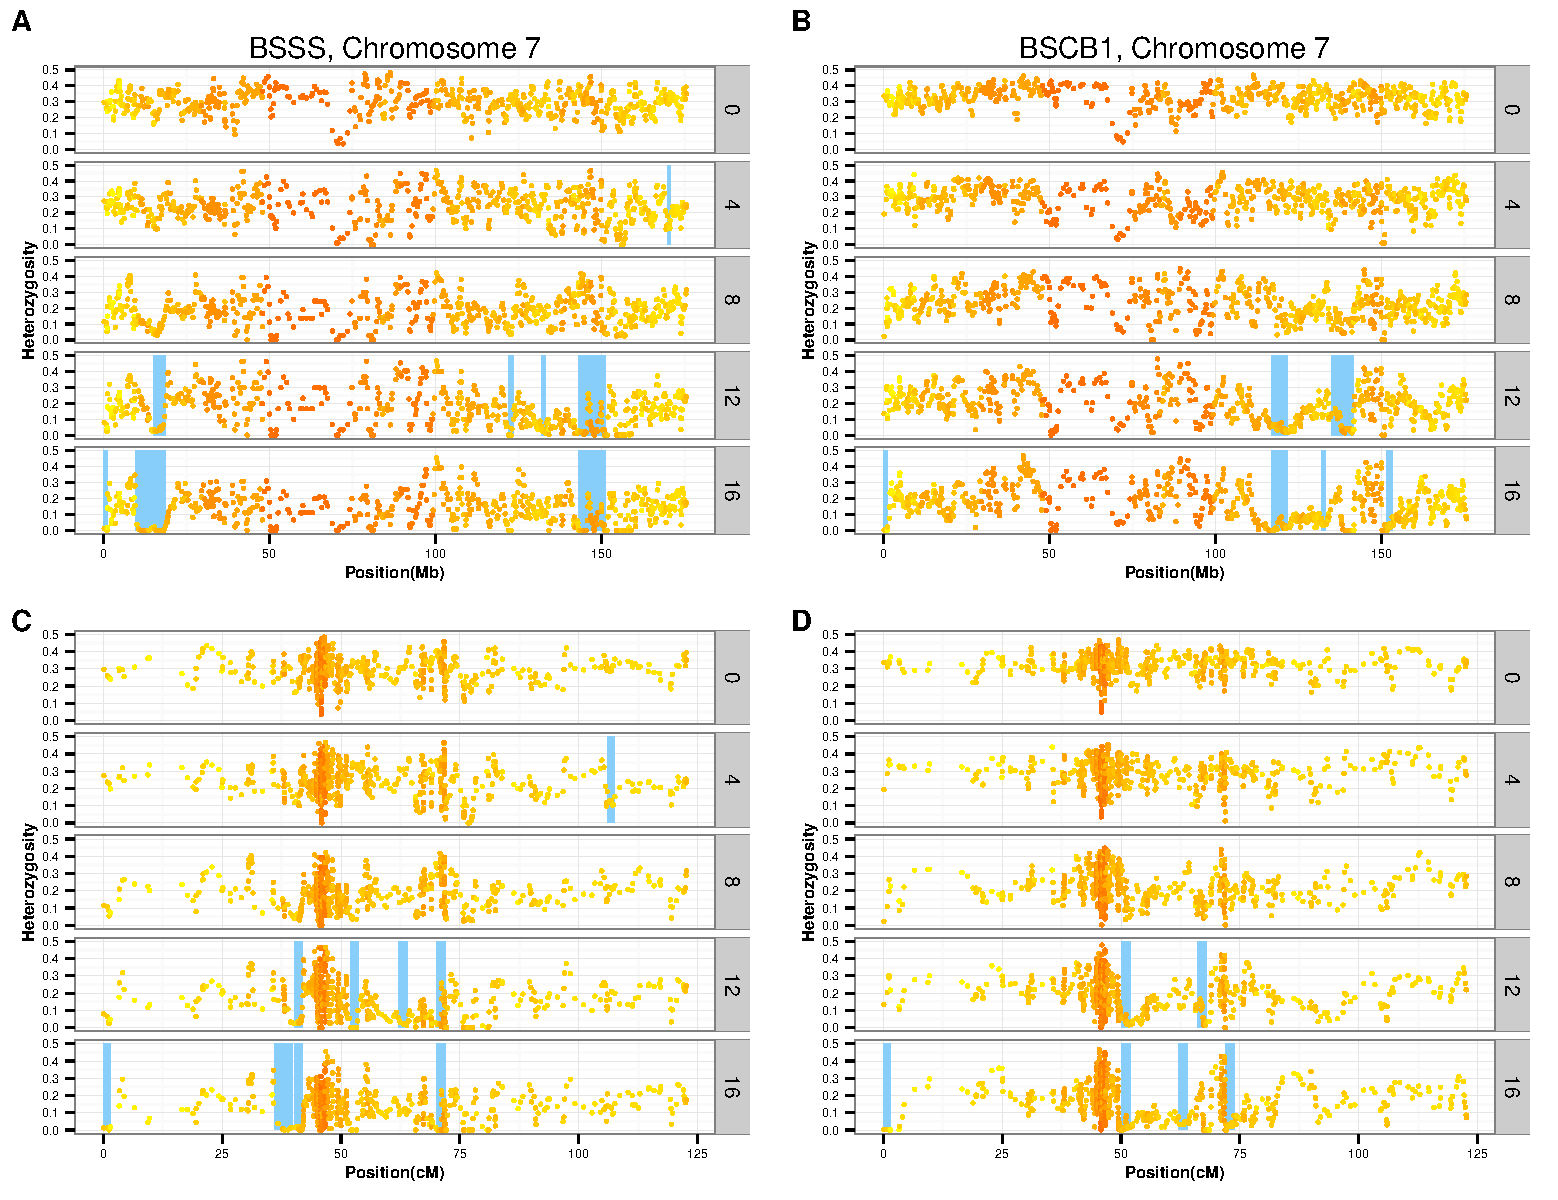
\includegraphics[width=0.7\linewidth]{Fig4/chrom7_combined.pdf}
%   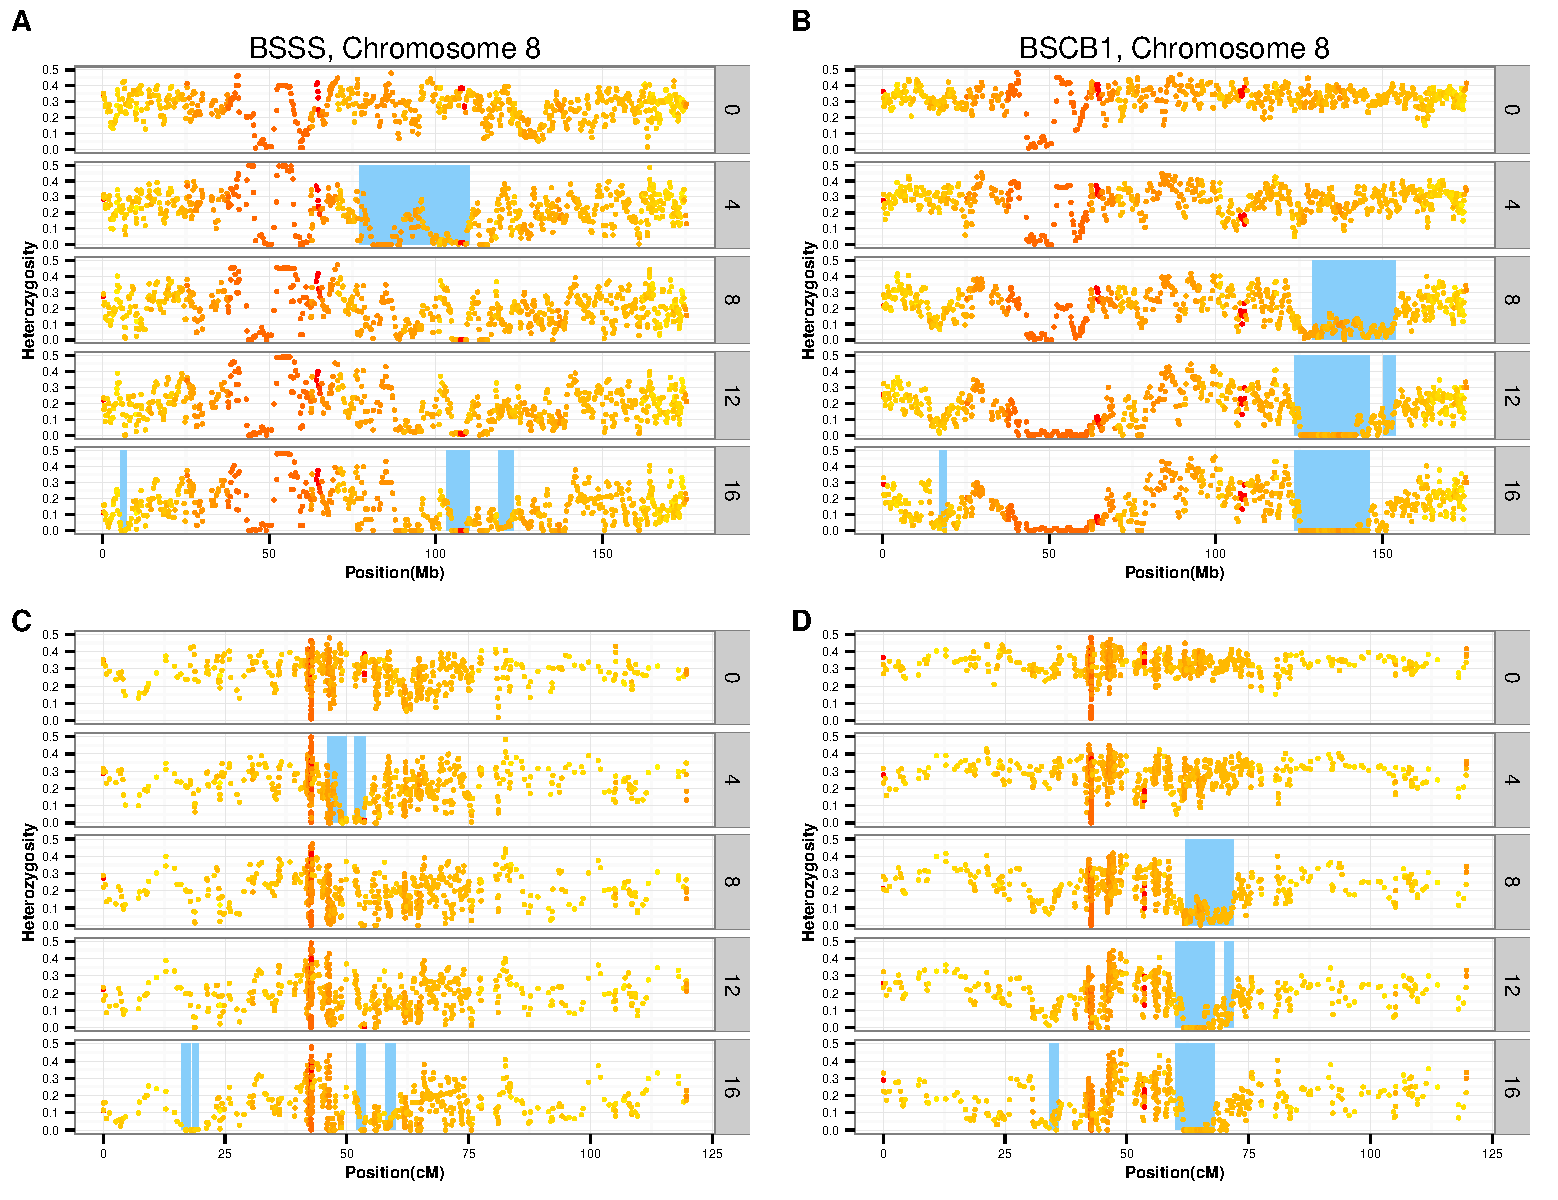
\includegraphics[width=0.7\linewidth]{Fig4/chrom8_combined.pdf}
%   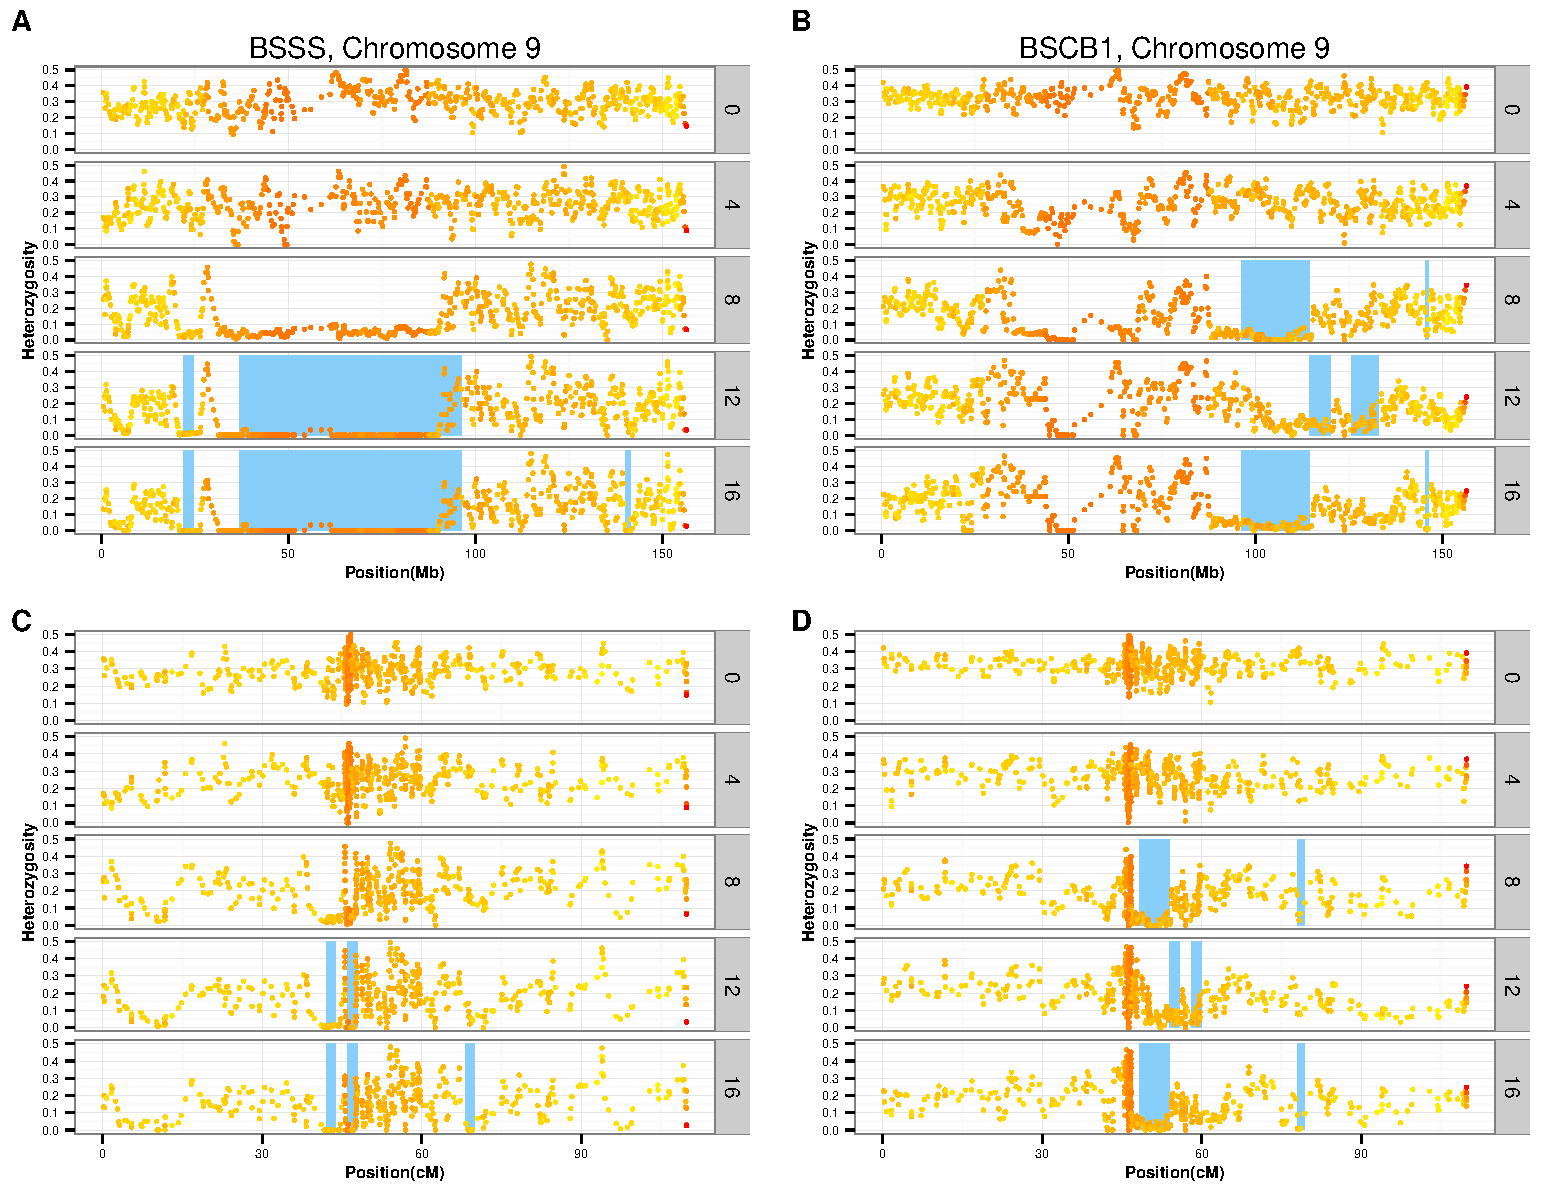
\includegraphics[width=0.7\linewidth]{Fig4/chrom9_combined.pdf}
%   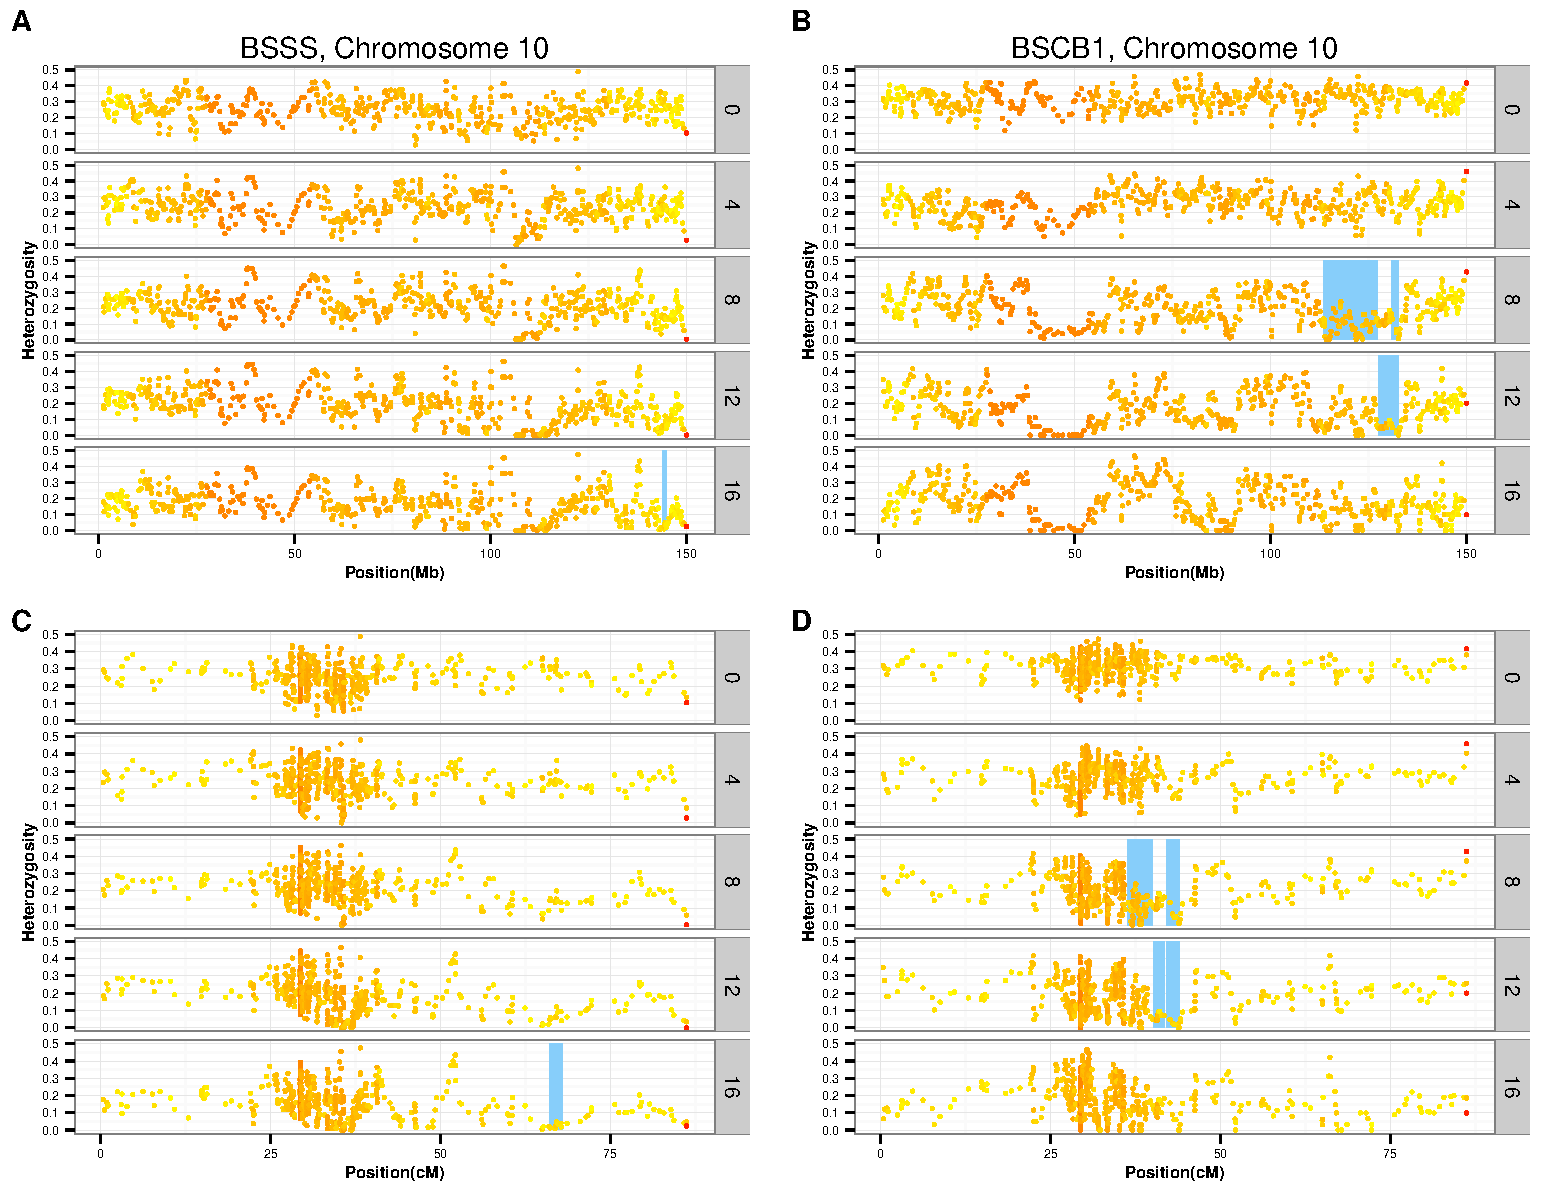
\includegraphics[width=0.7\linewidth]{Fig4/chrom10_combined.pdf}
%   %\renewcommand{\baselinestretch}{0.9}
%   \vspace{-3mm}
%   \caption{ Heterozygosity in each cycle across chromosomes of the BSSS (left) and BSCB1 (right) plotted on the physical (top) and genetic (bottom) map. Details are as in Fig. 4.
%} 
%\vspace{-6mm}
%    \label{fig:s2}
%  \end{center}
%\end{figure*}
%%%%%%%%%%%%%%%%%%%%%%%%%%%%%%%%%%%%%%%%%% FIGURE

\newpage

\begin{table}
\caption{Plants and Lines Genotyped in this study.
Backgrounds of the founder inbreds are from \citet{hagdorn2003molecular}}
\begin{tabular}{ | l | l | l | l | }

	{\bf Plants from the selection cycles} &  &  &  \\ 
	Population  & Cycle & \# plants &   \\ 
	BSSS & 0 & 34 &  \\ 
	BSSS & 4 & 36 &  \\ 
	BSSS & 8 & 35 &  \\ 
	BSSS & 12 & 36 &  \\ 
	BSSS & 16 & 36 &  \\ 
	BSCB1 & 0 & 36 &  \\ 
	BSCB1 & 4 & 36 &  \\ 
	BSCB1 & 8 & 35 &  \\ 
	BSCB1 & 12 & 36 &  \\ 
	BSCB1 & 16 & 36 &  \\ 
	 &  &  &  \\ 
	BSSS Founders Genotyped &  &  &  \\ 
	Inbred & Background / Pedigree &  &  \\ 
	Ind\_Tr9\_1\_1\_6 & Reid Early Dent (Troyer Strain) &  &  \\ 
	Oh3167B & Echelberger Clarage &  &  \\ 
	I224 & Iodent &  &  \\ 
	Ind467(744) & Reid Medium &  &  \\ 
	CI.187-2 & Krug-Nebraska Reid x IA Gold Mine &  &  \\ 
	Os420 & Osterland Yellow Dent &  &  \\ 
	I159 & Iodent &  &  \\ 
	A3G-3-1-3 & BL345BxIAI129 &  &  \\ 
	Ind\_Fe2\_1073* & Troyer Reid (Early) &  &  \\ 
	Ill\_Hy & IL High Yield &  &  \\ 
	Ill\_12E & unknown &  &  \\ 
	Ind\_AH83 & Funk 176A &  &  \\ 
	Ind\_B2* & Troyer Reid (Late Butler), parent of a founder &  &  \\ 
	LE23 & IL Low Ear &  &  \\ 
	*Parents of unavailable line F1B1 &  &  &  \\ 
	 &  &  &  \\ 
	BSCB1 Founders Genotyped &  &  &  \\ 
	Inbred & Background / Pedigree &  &  \\ 
	I205 & Iodent &  &  \\ 
	Oh51A & [(OH56xWf9)Oh56] (Wooster Clarage x ?) &  &  \\ 
	A340 & 4-29 x 64 (Silver King x Northwestern Dent) &  &  \\ 
	Ill\_Hy & IL High Yield &  &  \\ 
	Oh33 & Clarage &  &  \\ 
	Oh07 & C.I.540xIII.L &  &  \\ 
	R4 & Funk Yellow Dent &  &  \\ 
	Oh40B & eight line LSC composite &  &  \\ 
	P8 & Palin Reid &  &  \\ 
	L317 & LSC &  &  \\ 
	CC5 & Golden Glow (W23) &  &  \\ 
	 &  &  &  \\ 
	Founders not analyzed &  &  &  \\ 
	Inbred & Group & Reason &  \\ 
	CI.540 & BSSS & heterozygous genotype &  \\ 
	F1B1 & BSSS & unavailable &  \\ 
	CI.617 & BSSS & unavailable &  \\ 
	WD456 & BSSS & unavailable &  \\ 
	K230 & BSCB1 & source segregates phenotypically &  \\ 
	 &  &  &  \\ 
	Derived Lines Used &  &  &  \\ 
	Inbred & Group & Cycle & Notes \\ 
	B10 & BSSS & 0 & thrown out; poor data quality \\ 
	B42 & BSCB1 & 0 &  \\ 
	B14A & BSSS & 0 & Cuzco x B14 \\ 
	B43 & BSSS & 0 &  \\ 
	B10 & BSSS & 0 &  \\ 
	B37 & BSSS & 0 &  \\ 
	B44 & BSSS & 0 &  \\ 
	B17 & BSSS & 0 &  \\ 
	B69 & BSSS & 0 &  \\ 
	B39 & BSSS & 0 &  \\ 
	B90 & BSCB1 & 7 &  \\ 
	B40 & BSSS & 0 &  \\ 
	B54 & BSCB1 & 0 &  \\ 
	B78 & BSSS & 8 & from half-sib recurrent selection program \\ 
	B72 & BSSS & 3 & from half-sib recurrent selection program \\ 
	B84 & BSSS & 7 & from half-sib recurrent selection program \\ 
	B94 & BSSS & 8 &  \\ 
	B99 & BSCB1 & 10 &  \\ 
	B11 & BSSS & 0 &  \\ 
	B89 & BSSS & 7 &  \\ 
	B95 & BSCB1 & 7 &  \\ 
	B91 & BSCB1 & 8 &  \\ 
	B67 & BSSS & 0 &  \\ 
	B73 & BSSS & 5 & from half-sib recurrent selection program \\ 
	B97 & BSCB1 & 9 &  \\ 
	    \label{tab:s1}  % caption is needed to make this work
\end{tabular}
\end{table}
\newpage

\begin{table}
\caption{Evidence of minor contamination between cycles 4 and 8 in BSSS.}
\begin{tabular}{ | l | l | l | l | }
\hline
	\textbf{SNPs polymorphic in cycle} & \textbf{But not cycle} & \textbf{BSSS} & \textbf{BSCB1} \\ \hline
	4 & 0 & 290 & 225 \\ \hline
	8 & 0 & 2242 & 319 \\ \hline
	12 & 0 & 1227 & 181 \\ \hline
	16 & 0 & 344 & 128 \\ \hline
	8 & 4 & 4499 & 1081 \\ \hline
	12 & 4 & 2328 & 669 \\ \hline
	16 & 4 & 551 & 477 \\ \hline
	12 & 8 & 1821 & 1405 \\ \hline
	16 & 8 & 178 & 997 \\ \hline
	16 & 12 & 542 & 666 \\ \hline
	0 & Founders & 1202 & 1707 \\ \hline
	4 & Founders & 822 & 885 \\ \hline
	8 & Founders & 1201 & 798 \\ \hline
	12 & Founders & 816 & 550 \\ \hline
	16 & Founders & 445 & 460 \\ \hline
\end{tabular}
		    \label{tab:s2}  % caption is needed to make this work
\end{table}
\newpage

\begin{table}
\caption{Heterozygosity of SNPs in cycle 8 but not cycle 4 of the BSSS. }
\begin{tabular}{  l | l | l | }
\multicolumn{1}{l}{} & \multicolumn{1}{l}{BSSS} & \multicolumn{1}{l}{BSCB1}   \\ \cline{2-3}
	Mean & 0.052 & 0.052   \\ \cline{2-3}
	Median & 0.028 & 0.028   \\ \cline{2-3}
\end{tabular}
\end{table}
\jri{are  numbers in table supposed to be the same? I checked the Pages doc and they are the same there too.}
\jpg{yeah, it means one or two instances of the allele in a pop of 36.} 


\begin{table}
\caption{Switch error rates from computationally phasing ‘hybrids’ simulated from derived inbred lines.}
\begin{tabular}{ | l | l | l | l | l | l | }

\hline
	\textbf{Simulated 'Hybrid'} & \textbf{Derived Lines Used as Priors} & \textbf{Population} & \textbf{Possible Switches} & \textbf{Switch errors} & \textbf{Rate} \\ \hline
	B11xB67 & all & BSSS & 12195 & 41 & 0.003 \\ \hline
	B17xB44 & all & BSSS & 12230 & 58 & 0.005 \\ \hline
	B39xB37 & all & BSSS & 11485 & 129 & 0.011 \\ \hline
	B43xB69 & all & BSSS & 12266 & 26 & 0.002 \\ \hline
	B73xB72 & all & BSSS & 12043 & 47 & 0.004 \\ \hline
	B78xB94 & all & BSSS & 11658 & 51 & 0.004 \\ \hline
	B89xB84 & all & BSSS & 11517 & 53 & 0.005 \\ \hline
	B11xB67 & cycle 0 & BSSS & 12195 & 45 & 0.004 \\ \hline
	B17xB44 & cycle 0 & BSSS & 12230 & 54 & 0.004 \\ \hline
	B39xB37 & cycle 0 & BSSS & 11485 & 126 & 0.011 \\ \hline
	BB43xB69 & cycle 0 & BSSS & 12266 & 32 & 0.003 \\ \hline
	B42xB54 & all & BSCB1 & 11260 & 38 & 0.003 \\ \hline
	B90xB97 & all & BSCB1 & 6499 & 52 & 0.008 \\ \hline
	B91xB95 & all & BSCB1 & 7830 & 56 & 0.007 \\ \hline
	B99xB97 & all & BSCB1 & 6779 & 52 & 0.008 \\ \hline
	BB42xB54 & cycle 0 & BSCB1 & 11260 & 57 & 0.005 \\\hline
\end{tabular}
	\label{tab:s3}  % caption is needed to make this work
\end{table}